\begin{frame}
\frametitle{Quantum circuit}
\begin{columns}
  \begin{column}{0.5\textwidth}
    \begin{figure}
      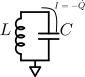
\includegraphics[scale=1.8]{LC_oscillator_annotated.pdf}
    \end{figure}
  \end{column}
  \begin{column}{0.5\textwidth}
    \begin{figure}
      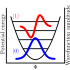
\includegraphics[scale=2.2]{wavefunctions.pdf}
    \end{figure}
  \end{column}
\end{columns}
\begin{columns}
  \begin{column}{0.5\textwidth}
    \begin{itemize}
      \item Superconductor
      \item no thermal occupation
      \item isolated from environment
      \item $\ddot{\Phi} = -\omega_0 \Phi$: harmonic oscillator
    \end{itemize}
    $\rightarrow$ quantum harmonic oscillator!
  \end{column}
  \begin{column}{0.5\textwidth}
    \begin{itemize}
      \item Quantized energy levels
      \item Wavefunctions in $\Phi$ and $Q$!
      \item (Bonus: How would you measure $\mathcolor{blue}{\ket{0}}$ versus $\mathcolor{red}{\ket{1}}$?)
    \end{itemize}
  \end{column}
\end{columns}
\end{frame}
